\chapter{Data structuren in Cassandra}
\label{ch:cassandra_data}
% row-oriented, maar toch columnfamily --> de kolommen worden opgeslaan in rijen
% SSTables and memtables

Bij Cassandra is er redelijk wat onduidelijkheid over de terminologie.
Dit komt omdat er twee implementaties, namelijk CQL en opslag, zijn.
Binnen deze twee implementaties worden vaak termen hergebruikt \citep{Ahmed2015Terminology}.
De structuren die hieronder besproken worden zijn allemaal onderdeel van de CQL implementatie.

\section{Column}
Binnen Cassandra is een kolom de kleinste datastructuur die er bestaat.
De kolom van een relationele database kan niet vergeleken worden met een kolom in Cassandra.
Hun functie is volledig anders.

\begin{figure}[H]
	\centering
	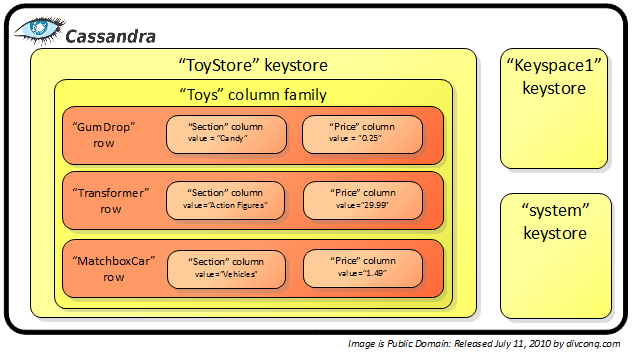
\includegraphics[width=0.75\textwidth]{img/4_data/column}
	\caption{Kolommen in Cassandra}
	\label{fig:column}
\end{figure}

Een kolom in Cassandra bevat drie of vier elementen:
\begin{enumerate}
	\item De naam van de kolom
	\item De waarde van de kolom
	\item Een timestamp
	\item Een time-to-live veld
\end{enumerate}

Voor de gebruiker zijn hier de naam van de kolom en de waarde van het grootste belang.
Met deze velden zal er uiteindelijk gewerkt worden.
De naam en waarde worden opgeslagen als byte arrays.
Toch voorziet Cassandra een resem built-in types.
De timestamp is er om conflicten op te lossen.
De time-to-live is een optioneel veld.
Hiermee kan aangegeven worden hoelang de kolom opgeslagen moet worden.

\section{Row}
Een rij kan beschouwd worden als een geordende lijst van kolommen.
Elke rij heeft een unieke sleutel.
Bij Cassandra is het zo dat als één kolom van een rij op een node staat, alle andere rijen ook op deze node staan.

Aan de hand van figuur \ref{ch:cassandra_data} kan verklaard worden waarom Cassandra tot de Column Family Store behoort, terwijl er toch sprake is van rijen.
De kolommen worden in Cassandra namelijk in rijen opgeslagen.

\section{Table}
Een niveau hoger dan de rij vindt men de tabel terug.
Binnen Cassandra is een tabel eigenlijk beter te beschrijven als een column family.
Dit was ook in de eerste versies van Cassandra het geval.

In een tabel vindt men alle rijen terug die hetzelfde schema hebben.
Toch kan Cassandra als een schemaloze database beschouwd worden doordat de kolommen zelf geen schema hoeven te hebben.
Door het feit dat men hier alle rijen groepeert is het belangrijk dat de rijen een unieke sleutel hebben \citep{hewitt2010cassandra}.

\section{Keyspace}
\label{sec:keyspace}
Een keyspace kan vergeleken worden met een database of schema in relationele databases.
De keyspace bevat de replicatiestrategie en replicatiefactor.

\begin{figure}[H]
	\centering
	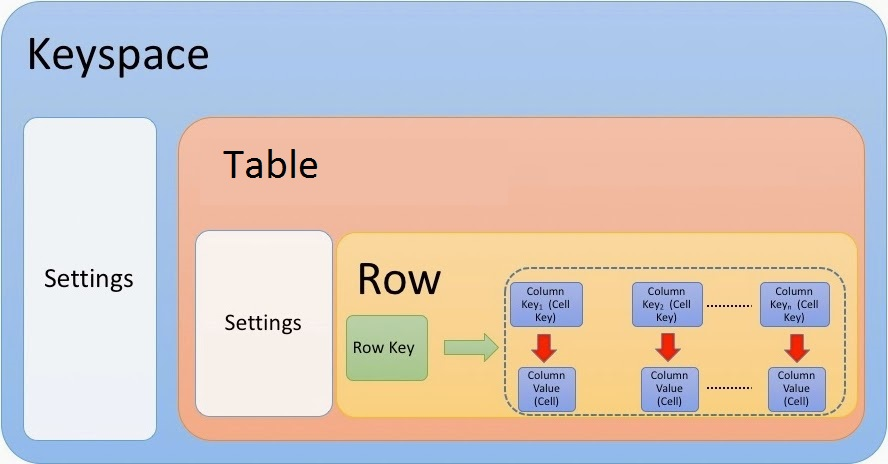
\includegraphics[width=0.7\textwidth]{img/4_data/data}
	\caption{Logische datastructuren in Cassandra}
	\label{fig:datastructure}
\end{figure}